\documentclass{beamer}
\usetheme{Madrid}

\usepackage{todonotes}
\usepackage{amsthm}
\usepackage{booktabs}
\usepackage{multirow}


\DeclareMathOperator*{\src}{src}
\DeclareMathOperator*{\dest}{dest}
\DeclareMathOperator*{\sgn}{sgn}


\newcommand{\notimplies}{%
\mathrel{{\ooalign{\hidewidth$\not\phantom{=}$\hidewidth\cr$\implies$}}}}


\newcommand{\localintersect}{\cap_{l}}
\newcommand{\indegree}{d_{\text{in}}}
\newcommand{\outdegree}{d_{\text{out}}}

\newcommand{\mainNS}{{\sc main}\xspace}
\newcommand{\articleNS}{{\sc article}\xspace}
\newcommand{\helpNS}{{\sc help}\xspace}
\newcommand{\userNS}{{\sc user}\xspace}
\newcommand{\usertalkNS}{{\sc user talk}\xspace}
\newcommand{\usercontrib}{{\sc user-contrib}\xspace}
\newcommand{\wikirfa}{{\sc wiki-Rfa}\xspace}
\newcommand{\posPR}{$\text{PR}_{\text{pos}}$\xspace}
\newcommand{\posF}{$\text{F1}_{\text{pos}}$\xspace}
\newcommand{\negF}{$\text{F1}_{\text{neg}}$\xspace}
\newcommand{\macroF}{$\text{F1}_{\text{macro}}$\xspace}
\newcommand{\negPR}{$\text{PR}_{\text{neg}}$\xspace}
\newcommand{\aucnegPR}{AUC-\negPR}
\newcommand{\aucposPR}{AUC-\posPR}
\newcommand{\iterStatus}{{\sc iterative-status}\xspace}
\newcommand{\plusrightarrow}{\xrightarrow{+}}
\newcommand{\minusrightarrow}{\xrightarrow{-}}
\newcommand{\plusleftarrow}{\xleftarrow{+}}
\newcommand{\minusleftarrow}{\xleftarrow{-}}

\AtBeginSection[]{
  \begin{frame}
  \vfill
  \centering
  \begin{beamercolorbox}[sep=8pt,center,shadow=true,rounded=true]{title}
    \usebeamerfont{title}\insertsectionhead\par%
  \end{beamercolorbox}
  \vfill
  \end{frame}
}


\usepackage{subcaption}
\usepackage{tikz}
\usetikzlibrary{positioning}
\usetikzlibrary{calc}
\usetikzlibrary{arrows}
\usetikzlibrary{arrows.meta}
\usetikzlibrary{decorations.pathmorphing,decorations.markings}
\usetikzlibrary{shapes}
\usetikzlibrary{patterns}
\usetikzlibrary{shadows,positioning}
\usepackage{amssymb}
\usepackage{amsmath}
\usepackage[ruled,linesnumbered]{algorithm2e}
\colorlet{colD}{red!40}
\colorlet{colIP}{cyan!40}
\colorlet{colV}{blue!40}
\colorlet{colBorder}{gray!70}


\title[Signed Vote Prediction]{Vote Prediction Models for Signed Social Networks}
\author{Ananth Mahadevan}
\institute{Aalto University}
\date{\today}

\begin{document}
\begin{frame}
    \titlepage
\end{frame}

\begin{frame}
    \frametitle{Overview}
    \tableofcontents
\end{frame}


\section{Voting and Signed Networks}

\begin{frame}
    \frametitle{Voting in Communities}
    \begin{itemize}
        \item Communities need to take collective action 
        \item Voting is a popular method 
        \item Members of the community vote on the agenda
        \item For example
        \begin{itemize}
            \item Politicians voting for bills in the parliament
            \item Wikipedia users voting for promoting administrators 
        \end{itemize}
        \item Understanding voting behaviour is beneficial
        \begin{itemize}
            \item Can propose agendas items which will be successful 
            \item Identify ideological fault lines amongst members
        \end{itemize}
    \end{itemize}
    
\end{frame}

\begin{frame}
    \frametitle{Votes as Signed Graphs}
    \begin{itemize}
        \item Votes are usually \textbf{for} or \textbf{against} an agenda
        \item Intuitively maps to \textbf{positive} and \textbf{negative} edges in signed graphs 
        \item More tools to analyse voting patterns, e.g.,
        \begin{itemize}
            \item Correlation clustering \cite{brito2020aBrazil,arinik2017signed}
            \item Balance and Status \cite{levorato2016brazilian,derr2018congressional}
        \end{itemize}
        \item Two main prediction tasks exist with regard to voting 
        \begin{enumerate}
            \item Predicting the result
            \item Predicting an individual vote
        \end{enumerate}
        \item We focus on predicting votes
    \end{itemize}
    
\end{frame}

\begin{frame}
    \frametitle{Predicting Votes}
    Predicting a vote can be split into two phases
    \begin{enumerate}
        \item \textbf{Who} will vote next
        \begin{itemize}
            \item Same as link prediction task
            \item Is trivial when voting order is known, e.g., parliament roll calls
            \item Combinatorial if no known underlying process
        \end{itemize}
        \item \textbf{How} they will vote 
        \begin{itemize}
            \item Same as sign prediction task
            \item Triad features encode balance and status theory
            \item Train a supervised ML model using network and triad features \cite{leskovec2010predicting,leskovec2010signed}
        \end{itemize}
    \end{enumerate}
    We propose an \textit{unsupervised iterative model} to predict the sign of a vote using balance and status theory.

\end{frame}

\section{Wikipedia Elections}
\begin{frame}
    \frametitle{Requests for Adminship (RfA)}    
    \begin{itemize}
        \item RfAs are an election-esque process to gain admin rights
        \item Anyone can nominate a \textbf{candidate} or self-nominate
        \item 7 day long period of voting and discussion
        \item Any registered editor can comment and vote :
        \begin{itemize}
            \item Support 
            \item Oppose
            \item Neutral
        \end{itemize}
        \item Highly intense process with Q\&A with the candidate about Wiki policy etc
        \item Final decision is made by a Bureaucrat (a special class of users)
        \item Decision is based on if a \textbf{consensus} has been reached
        \item Successful RfAs usually have 75\% support
    \end{itemize}


\end{frame}

\section{Local Signed Network}
\begin{frame}
    \frametitle{Terminology}
    \begin{itemize}
        \item Current voting session is a signed graph $S=(V_S,E_S,w_S)$
        \item It contains current voter $v$, candidate $c$ and prior set of voters $U$
        \item We also have a signed \textit{Relationship Graph}, $R = (V_R,E_R,w_R)$
        \item It is created from the historical voting data, $H$
        \item The \textit{Local Signed Network} is defined as $LSN = ( V_S \cap V_R, E_S\cup E_R)$
        \item Essentially the subgraph of the voter's neighbours in $R$, who have already voted in $S$
        \item Can use balance and status theory in the LSN to predict votes
    \end{itemize}
    

\end{frame}


\section{Balance Theory}

\subsection{Agreement Graph}
\begin{frame}
    \frametitle{Balance Theory}
    \begin{itemize}
        \item Balance theory works for undirected signed graphs
        \item A cycle is balanced if it has even number of negative links
        \item A graph is balanced iff every cycle is balanced
        \item Triads $B_1$, $B_2$ are balanced
        \item Triads $B_3$ and $B_4$ are unbalanced
    \end{itemize}
    \begin{figure}
        \centering
        \scalebox{0.75}{\tikzset{
    position/.style args={#1:#2 from #3}{
        at=(#3.#1), anchor=#1+180, shift=(#1:#2)
    }
}

\begin{tikzpicture}

    \begin{scope}[every node/.style={circle,thick,draw}]
        \node (v1) at (0,0) {};
        \node[position=-120:1cm from v1] (v2) {};
        \node[position=-60:1cm from v1] (v3) {};
        
        \node[right=2cm of v1] (v4) {};
        \node[position=-120:1cm from v4] (v5) {};
        \node[position=-60:1cm from v4] (v6) {};
        
        \node[right=2cm of v4] (v7) {};
        \node[position=-120:1cm from v7] (v8) {};
        \node[position=-60:1cm from v7] (v9) {};
        
        \node[right=2cm of v7] (v10) {};
        \node[position=-120:1cm from v10] (v11) {};
        \node[position=-60:1cm from v10] (v12) {};
        

    \end{scope}

    \begin{scope}[>={Stealth[red]},
        positive/.style={thick,draw},
        negative/.style={thick,dashed,draw},
        every node/.style={fill=white,circle}]
        % \draw (v4) -- (v1) -- (v3) -- (v2) -- (v1);
        \path 
        (v1) edge[positive] node[above left=0.1mm and 0.1mm] {$+$} (v2)
        (v1) edge[positive] node[above right=0.1mm and 0.1mm] {$+$} (v3) 
        (v3) edge[positive] node[below] {$+$} node[below=1cm] {$T_1$}  (v2)      
        ;
        \path 
        (v4) edge[negative] node[above left=0.1mm and 0.1mm] {$-$} (v5)
        (v4) edge[negative] node[above right=0.1mm and 0.1mm] {$-$} (v6) 
        (v6) edge[positive] node[below] {$+$} node[below=1cm] {$T_2$}  (v5)      
        ;
        \path 
        (v7) edge[positive] node[above left=0.1mm and 0.1mm] {$+$} (v8)
        (v7) edge[positive] node[above right=0.1mm and 0.1mm] {$+$} (v9) 
        (v9) edge[negative] node[below] {$-$} node[below=1cm] {$T_3$}  (v8)      
        ;
        \path 
        (v10) edge[negative] node[above left=0.1mm and 0.1mm] {$-$} (v11)
        (v10) edge[negative] node[above right=0.1mm and 0.1mm] {$-$} (v12) 
        (v12) edge[negative] node[below] {$-$} node[below=1cm] {$T_4$}  (v11)      
        ;
    \end{scope}
  \end{tikzpicture}
  }
    \end{figure}

\end{frame}

\begin{frame}
    \frametitle{Agreement Graph}
    \begin{itemize}
        \item Define a symmetric relationship based on \textbf{agreement} 
        \item Subtract 0.5 from agreement ratio to get a signed measure
        \item Create an \textit{Agreement Graph}, $A=(V_A,E_A,w_A)$
    \end{itemize}
    \begin{block}{Signed Symmetric Measure}
        $$w_{A}((u,v)) = \frac{\text{Number of times } u \text{ and } v \text{ have voted similarly}}{\text{Number of common RfAs for } u \text{ and } v} -0.5$$
    \end{block}

\end{frame}

\begin{frame}
    \frametitle{How to measure balance?}
    \begin{itemize}
        \item Triads can capture local balance of a network
        \item Need to capture information from longer cycles \cite{chiang2011exploiting}
        \item Smallest eigenvalue $\lambda_{1}$ of the signed Laplacian $\overline{L}$ is a measure of the imbalance of the network \cite{hou2005bounds}
        \item  We state that a voter chooses to maintain the balance of the LSN
        \item Therefore, can use $\lambda_{1}$ as the basis for predictions in the model
    \end{itemize}
    

\end{frame}
\subsection{Model}
\begin{frame}
    \frametitle{Iterative Balance Model}
    \centering
    \scalebox{0.7}{\tikzset{
        position/.style args={#1:#2 from #3}{
            at=(#3.#1), anchor=#1+180, shift=(#1:#2)
        }
    }

\begin{figure}[!ht]
    \centering

\begin{tikzpicture}

    \begin{scope}[every node/.style={circle,thick,draw,minimum size=9mm}]
        \node (u1) at (0,0) {$u_1$};
        \node[position=-60:1.3cm from u1] (c) {$c$};
        \node[position=-120:1.3cm from u1] (v) {$v$};

        \node[right= 5cm of u1] (u2) {$u_2$};
        \node[left=1cm of u2] (u12) {$u_1$};
        \node[position=-90:1cm from u2] (c2) {$c$};
        \node[left=1cm of c2] (v2) {$v$};

        \path (c) -- node[below=3cm] (u3) {$u_3$} (v2); 
        \node[right= 1cm of u3] (u13) {$u_1$};
        \node[below=1cm of u3] (c3) {$c$};
        \node[right=1cm of c3] (u23) {$u_2$};
        \node[left=1cm of c3] (v3) {$v$};
    \end{scope}

    % positive edges
    \begin{scope}[
        relation/.style= {thick,draw,blue},
        vote/.style= {very thick,draw,red,densely dotted},
        predict/.style={thick,draw,dashed},
        every node/.style={fill=white,rectangle,inner sep=0}]
        % \draw (v4) -- (v1) -- (v3) -- (v2) -- (v1);
        \path 
        (u1) edge[vote] node[above right=1mm] {$-$} (c)  
        (v) edge[relation] node[above left=1mm] {$-$} (u1)
        (v) edge[predict] (c)
        
        (u12) edge[vote] node[above right=1mm] {$-$} (c2)  
        (u2) edge[vote] node[right=1mm] {$+$} (c2)
        (u2) edge[relation] node[above=1mm] {$-$} (u12)
        (v2) edge[relation] node[left=1mm] {$+$} (u12)
        (v2) edge[predict] (c2)

        (u13) edge[vote] node[above left=1mm] {$-$} (c3)  
        (u23) edge[vote] node[above=1mm] {$+$} (c3)
        (u3) edge[vote] node[left=1mm] {$-$} (c3)
        (u23) edge[relation] node[right=1mm] {$-$} (u13)
        (u3) edge[relation] node[above=1mm] {$+$} (u13)
        (v3) edge[relation] node[above left=1mm] {$-$} (u3)
        (v3) edge[relation,bend right=50] node[above=1mm] {$-$} (u23)
        (v3) edge[predict] (c3)

        
        ;
    \end{scope}
    \begin{scope}[
        every edge/.style= {},
        every node/.style={fill=white,rectangle,inner sep=0,text=black}]
    \path 
    (v) edge node[below=2cm] {$(a)~i=1$} (c)
    (v) edge node[below=1cm] {$\lambda_1^+ = 0, \lambda_1^-=1$} (c)
    
    (v2) edge node[below=2cm] {$(b)~i=2$} (c2)
    (v2) edge node[below=1cm] {$\lambda_1^+ = 0.58, \lambda_1^-=0$} (c2)
    (v3) edge node[below=3cm] {$(c)~i=3$} (u23)
    (v3) edge node[below=2cm] {$\lambda_1^+ = 0.55, \lambda_1^-=0.55$} (u23)
    ;
    \end{scope}
  \end{tikzpicture}
  


    \caption{Local Singed Network prediction based on balance theory. At every iteration $i$ the dotted red lines are prior votes, solid blue lines are relationships based on voting records and the dashed black edge $(v,c)$ is the edge whose sign is being predicted. $\lambda_1^+$ and $\lambda_1^-$ correspond to the smallest eigenvalue of the signed Laplacian $\overline{L}_i$ based on whether $w((v,c))=+1$ or $w((v,c))=-1$.     }
    \label{}
\end{figure}}

\end{frame}

\section{Status Theory}


\subsection{Follows Graph}

\begin{frame}
    \frametitle{Status Theory}
    \begin{itemize}
        \item Status theory is based on relative merit of nodes
        \item Edge $u\plusrightarrow v$ : $v$ has higher status than $u$
        \item Edge $u \minusrightarrow v$ : $v$ has lower status than $u$
        \item Status and Balance theories can contradict each other when used to predict edges
        \item Triads $S_2$, $S_3$ and $S_4$ adhere to status theory
        \item Only triads $S_1$ and $S_3$ are balanced 
    \end{itemize}
    \begin{figure}
        \centering
        \scalebox{0.7}{\tikzset{
    position/.style args={#1:#2 from #3}{
        at=(#3.#1), anchor=#1+180, shift=(#1:#2)
    }
}

\begin{tikzpicture}

    \begin{scope}[every node/.style={circle,thick,draw}]
        \node (v2) at (0,0) {$v_2$};
        \node[position=-120:1cm from v2] (v1) {$v_1$};
        \node[position=-60:1cm from v2] (v3) {$v_3$};
        
        \node[right=2.5cm of v2] (v5) {$v_2$};
        \node[position=-120:1cm from v5] (v4) {$v_1$};
        \node[position=-60:1cm from v5] (v6) {$v_3$};
        
        \node[right=2.5cm of v5] (v8) {$v_2$};
        \node[position=-120:1cm from v8] (v7) {$v_1$};
        \node[position=-60:1cm from v8] (v9) {$v_3$};
        
        \node[right=2.5cm of v8] (v11) {$v_2$};
        \node[position=-120:1cm from v11] (v10) {$v_1$};
        \node[position=-60:1cm from v11] (v12) {$v_3$};
        

    \end{scope}

    \begin{scope}[>={Stealth[black]},
        positive/.style={thick,draw,->},
        negative/.style={thick,dashed,draw,->},
        every node/.style={fill=white,circle}]
        % \draw (v4) -- (v1) -- (v3) -- (v2) -- (v1);
        \path 
        (v1) edge[positive] node[above left=0.1mm and 0.1mm] {$+$} (v2)
        (v2) edge[positive] node[above right=0.1mm and 0.1mm] {$+$} (v3) 
        (v3) edge[positive] node[below] {$+$} node[below=1cm] {$S_1$}  (v1)      
        ;
        \path 
        (v4) edge[positive] node[above left=0.1mm and 0.1mm] {$+$} (v5)
        (v5) edge[positive] node[above right=0.1mm and 0.1mm] {$+$} (v6) 
        (v6) edge[negative] node[below] {$-$} node[below=1cm] {$S_2$}  (v4)      
        ;
        \path 
        (v7) edge[positive] node[above left=0.1mm and 0.1mm] {$+$} (v8)
        (v8) edge[negative] node[above right=0.1mm and 0.1mm] {$-$} (v9) 
        (v9) edge[negative] node[below] {$-$} node[below=1cm] {$S_3$}  (v7)      
        ;
        \path 
        (v10) edge[positive] node[above left=0.1mm and 0.1mm] {$+$} (v11)
        (v11) edge[negative] node[above right=0.1mm and 0.1mm] {$-$} (v12) 
        (v12) edge[positive] node[below] {$+$} node[below=1cm] {$S_4$}  (v10)      
        ;
    \end{scope}
  \end{tikzpicture}
  }
    \end{figure}

\end{frame}

\begin{frame}
    \frametitle{Follows Graph}
    \begin{itemize}
        \item Define an asymmetric relationship based on \textbf{following} 
        \item Create an \textit{Follow Graph}, $F=(V_F,E_F,w_F)$
        \item An edge $u \rightarrow v$ indicates $u$ votes after $v$
        \item Weight is 0.5 subtracted from the \textit{follower ratio}
    \end{itemize}
    \begin{block}{Signed Asymmetric Measure}
        $$ w_{F}((u,v)) = \frac{\text{Number of times } u \text{ voted after and agreed with } v }{\text{Number of times } u \text{ voted after } v} -0.5$$
    \end{block}

\end{frame}


\subsection{Agony and Status}

\begin{frame}
    \frametitle{How to measure status?}
    \begin{itemize}
        \item Directed triads and other graph motifs can be a proxy for measuring status \cite{Liu2019LinkPrediction}
        \item Heuristic for status like  $\sigma(v) = \indegree^{+}(v) + \outdegree^{-}(v) - \outdegree^{+}(v)- \indegree^{-}(v)$ \cite{leskovec2010predicting}
        \item These still only capture local effect of status
        \item Cannot measure violations of status in larger cycles
        \item The concept of a nodes possessing an implicit status is very similar to a \textbf{hierarchy} 
    \end{itemize}
\end{frame}

\begin{frame}
    \frametitle{Agony}
    \begin{itemize}
        \item Assume a ranking for nodes, $r:V\rightarrow \mathbb{N}$
        \item An edge $u \rightarrow v$ causes \textbf{agony}, if $r(u)\geq r(v)$
        \item Quantified as $\max(r(u)-r(v)+1,0)$ for an edge
        \item Agony of a graph $G$ wrt $r$ is $A(G,r) =  \sum_{(u,v)\in E} \max(r(u)-r(v)+1,0)$
        \item Agony of a graph is the lowest possible agony over all rankings $A(G) = \min_{r\in \text{Rankings}}A(G,r)$
        \item Lower agony means better hierarchy, $h(G)=1-\frac{1}{|E|}A(G)$
    \end{itemize}
\end{frame}

\begin{frame}
    \frametitle{Examples}
    \begin{figure}[!ht]
        \centering
        \begin{subfigure}[t]{0.5\textwidth}
            \centering
            \scalebox{0.5}{\tikzset{
    position/.style args={#1:#2 from #3}{
        at=(#3.#1), anchor=#1+180, shift=(#1:#2)
    }
}

\begin{tikzpicture}

    \begin{scope}[every node/.style={circle,thick,draw}]
        \node (v1) at (0,0) {$1$};
        \node[right=1.5cm of v1] (v2) {$1$};
        \node[right=1.5cm of v2] (v3) {$1$};
        \node[above=1cm of v2] (v5) {$2$};
        \node[left=3cm of v5] (v4) {$2$};
        \node[right=2.5cm of v5] (v6) {$2$};
        \node[above right=1cm and 1.5cm of v4] (v7) {$3$};
        \node[above=2cm of v4] (v8) {$4$};
        \node[right=5cm of v8] (v9) {$4$};
    \end{scope}

    \begin{scope}[>={Stealth[black]},
        every edge/.style={thick,draw,->},
        every node/.style={fill=white,circle}]
        % \draw (v4) -- (v1) -- (v3) -- (v2) -- (v1);
        \path 
        (v1) edge (v4)
        (v1) edge (v7)
        (v1) edge (v5)
        (v2) edge (v5)
        (v3) edge (v5)
        (v3) edge (v6)
        (v3) edge (v9)
        (v4) edge (v7)
        (v4) edge (v8)
        (v5) edge (v7)
        (v6) edge (v9)
        (v7) edge (v8)
        (v7) edge (v9)

        ;
    \end{scope}
  \end{tikzpicture}
  }
            \caption{DAG has perfect hierarchy, $h(G)=1$ and agony of each edge is 0}
            \label{fig:dag}
        \end{subfigure}

        \begin{subfigure}[t]{0.4\textwidth}
            \centering
            \scalebox{0.5}{\tikzset{
    position/.style args={#1:#2 from #3}{
        at=(#3.#1), anchor=#1+180, shift=(#1:#2)
    }
}

\begin{tikzpicture}

    \begin{scope}[every node/.style={circle,thick,draw}]
        \node (v1) at (0,0) {$1$};
        \node[right=1.5cm of v1] (v2) {$1$};
        \node[above=1.5cm of v2] (v3) {$1$};
        \node[left=1.5cm of v3] (v4) {$1$};

    \end{scope}

    \begin{scope}[>={Stealth[black]},
        every edge/.style={thick,draw,->},
        every node/.style={fill=white,circle}]
        % \draw (v4) -- (v1) -- (v3) -- (v2) -- (v1);
        \path 
        (v1) edge (v2)
        (v2) edge (v3)
        (v3) edge (v4)
        (v4) edge (v1)

        ;
    \end{scope}
  \end{tikzpicture}
  }
            \caption{A cycle has no hierarchy, $h(G)=0$ and each edge has agony of 1}
            \label{fig:cycle}
        \end{subfigure}
        \hspace{4mm}%
        \begin{subfigure}[t]{0.4\textwidth}
            \centering
            \scalebox{0.5}{\tikzset{
    position/.style args={#1:#2 from #3}{
        at=(#3.#1), anchor=#1+180, shift=(#1:#2)
    }
}

\begin{tikzpicture}

    \begin{scope}[every node/.style={circle,thick,draw}]
        \node (v1) at (0,0) {$1$};
        \node[right=2cm of v1] (v2) {$1$};
        \node[above right=1.5cm of v1] (v3) {$2$};
        \node[above left = 1.5cm of v3] (v4) {$3$};
        \node[above right=1.5cm of v3] (v5) {$3$};
    \end{scope}

    \begin{scope}[>={Stealth[black]},
        every edge/.style={thick,draw,->},
        back/.style ={very thick,dashed,red,->},
        every node/.style={fill=white,circle}]
        % \draw (v4) -- (v1) -- (v3) -- (v2) -- (v1);
        \path 
        (v1) edge (v3)
        (v1) edge (v4)
        (v2) edge (v3)
        (v3) edge (v5)
        (v5) edge[back,bend left] (v2)
        ;
    \end{scope}
  \end{tikzpicture}
  }
            \caption{Graph with some hierarchy $h(G)=2/5$. Red dashed edge has agony of 3 and solid black edges have 0 agony.  }
            \label{fig:some-hierarchy}
        \end{subfigure}
        \caption{Examples of hierarchy in unweighted directed graphs. Numbers inside nodes indicate the rank of vertex.}
        \label{fig:hierarchy} 
    \end{figure}
\end{frame}

\begin{frame}
    \frametitle{Agony and Status}
    \begin{itemize}
        \item \cite{gupte2011finding} and \cite{tatti2017tiers} provide algorithms to compute agony of directed graphs
        \item Consider rank function $r$ as status function $\sigma$
        \item For an edge $u \rightarrow v$, $\sigma(u)\geq\sigma(v)$ is a status violation
        \item Therefore, agony is a measure of status violation of an edge
        \item The agony of a network is the \textbf{overall status compliance} of $G$
        \item What to do with signed edges?
        \begin{itemize}
            \item Flip edges $u \minusrightarrow v$ to $u \plusleftarrow v$
        \end{itemize}
        \item Now, we say a voter chooses to reduce the agony of the LSN
    \end{itemize}

\end{frame}

\subsection{Model}
\begin{frame}
    \frametitle{Iterative Status Model}
        \centering
        \scalebox{0.5}{\tikzset{
        position/.style args={#1:#2 from #3}{
            at=(#3.#1), anchor=#1+180, shift=(#1:#2)
        }
    }

\begin{figure}[!ht]
    \centering

\begin{tikzpicture}

    \begin{scope}[every node/.style={circle,thick,draw,minimum size=9mm}]
        \node (u) at (0,0) {$u$};
        \node[position=-60:1.3cm from u] (c) {$c$};
        \node[position=-120:1.3cm from u] (v) {$v$};
        
        \node[position=-120:2cm from v] (u1)  {$u$};
        \node[position=-60:1.3cm from u1] (c1) {$c$};
        \node[position=-120:1.3cm from u1] (v1) {$v$};

        \node[position=-60:2cm from c] (u2)  {$u$};
        \node[position=-60:1.3cm from u2] (c2) {$c$};
        \node[position=-120:1.3cm from u2] (v2) {$v$};

        \node[position=-90:4cm from u1] (u3)  {$u$};
        \node[position=-60:1.3cm from u3] (c3) {$c$};
        \node[position=-120:1.3cm from u3] (v3) {$v$};

        \node[position=-90:4cm from u2] (u4)  {$u$};
        \node[position=-60:1.3cm from u4] (c4) {$c$};
        \node[position=-120:1.3cm from u4] (v4) {$v$};


    \end{scope}

    % positive edges
    \begin{scope}[
        relation/.style= {thick,draw,blue,->,>={Stealth[blue]}},
        vote/.style= {very thick,draw,red,densely dotted,->,>={Stealth[red]}},
        predict/.style={thick,draw,dashed,->,>={Stealth[black]}},
        assume/.style={thick,draw,->,>={Stealth[black]}},
        every node/.style={fill=white,rectangle,inner sep=0}]
        % \draw (v4) -- (v1) -- (v3) -- (v2) -- (v1);
        \path 
        (u) edge[vote] node[above right=1mm] {$-$} (c)  
        (v) edge[relation] node[above left=1mm] {$-$} (u)
        (v) edge[predict] (c)

        (u1) edge[vote] node[above right=1mm] {$-$} (c1)  
        (v1) edge[relation] node[above left=1mm] {$-$} (u1)
        (v1) edge[assume] node[above=1mm] {$+$} (c1)
        
        (u2) edge[vote] node[above right=1mm] {$-$} (c2)  
        (v2) edge[relation] node[above left=1mm] {$-$} (u2)
        (v2) edge[assume] node[above=1mm] {$-$} (c2)
        
        (c3) edge[vote] node[above right=1mm] {$+$} (u3)  
        (u3) edge[relation] node[above left=1mm] {$+$} (v3)
        (v3) edge[assume] node[above=1mm] {$+$} (c3)
        
        (c4) edge[vote] node[above right=1mm] {$+$} (u4)  
        (u4) edge[relation] node[above left=1mm] {$+$} (v4)
        (c4) edge[assume] node[above=1mm] {$+$} (v4)
        ;
    \end{scope}
    \begin{scope}[
        every edge/.style= {thick,draw,->},
        every node/.style={fill=white,rectangle,inner sep=0,text=black}
    ]
    \node[position=-90:4cm from u3] (a1) {$\alpha^+=3$};
    \node[position=-90:4cm from u4] (a2) {$\alpha^-=0$};
    \path     
    (v) edge[shorten >=0.5cm,shorten <=0.5cm] node[above left=0.1cm,text width=2cm,align=center] {Assume \\ positive vote} (u1)
    (c) edge[shorten >=0.5cm,shorten <=0.5cm] node[above right=0.1cm,text width=2cm,align=center] {Assume \\ Negative vote} (u2)

    ($(u1)!0.5!(u3)$) edge node[right=1mm] (convertL) {} ($(u1)!0.8!(u3)$)
    ($(u2)!0.5!(u4)$) edge node[left=1mm] (convertR) {} ($(u2)!0.8!(u4)$)
    
    (convertL) edge[draw=none] node[text width=3cm,align=center] {Transform\\ negative edges} (convertR)
    
    ($(u3)!0.6!(a1)$) edge node[right=1mm] (agonyL) {} ($(u3)!0.9!(a1)$)
    ($(u4)!0.6!(a2)$) edge node[left=1mm] (agonyR) {} ($(u4)!0.9!(a2)$)
    
    (agonyL) edge[draw=none] node[text width=3cm,align=center] {Compute\\ Agony} (agonyR)

    ;
    \end{scope}
  \end{tikzpicture}
  


    \caption{Example of LSN sign prediction using status theory.}
    \label{fig:lsn-status}
\end{figure}}
    

\end{frame}

\section{Iterative Prediction}

\begin{frame}
    \frametitle{Iterative Predictions and its Advantages}
    \begin{itemize}
        \item Predictions with balance and status are unsupervised
        \item Can be bootstrapped by starting with an empty graph $R$
        \item After predicting votes in a session, it updates $R$
        \item Iteratively gathers more information in $R$, increasing performance
        \item Therefore, the model can be trained on the entire dataset
    \end{itemize}
    

\end{frame}
\begin{frame}
    \frametitle{Algorithm}
    \centering
    \scalebox{0.7}{
    \begin{algorithm}[H]
        \DontPrintSemicolon
        \KwIn{Candidate $c$, Relationship graph $R=(V_R,E_R,w_R)$, Order of voters in current session $O$ and true votes $w^*$  }
        \KwResult{Predictions for current session }
        $k \leftarrow |O|$\;
        $u \leftarrow O[1]$ \tcp*{First voter} 
        $V_S \leftarrow \{c,u\}$ \tcp*{candidate and first voter}
        $E_S \leftarrow \{(u,c)\}$ \tcp*{first vote}
        $w_S((u,c)) \leftarrow w^{*}((u,c))$ \tcp*{Assign true vote}
        Initialize session graph $S = \{V_S,E_S,w_S\}$\;
        $predictions \leftarrow \emptyset$ \;
        \For{$i \leftarrow 2$ \KwTo $k$}{
            $v \leftarrow O[i]$\; 
            $V_S \leftarrow V_S \cup \{v\}$ \;
            $LSN \leftarrow S \cap R$\;
            $p \leftarrow Predict(v,c,LSN)$\; 
            $predictions \leftarrow predictions \cup p$\;
            $E_S \leftarrow E_S \cup \{(v,c)\}$\;
            $w_S((v,c)) \leftarrow w^{*}((v,c))$ \tcp*{Assign true vote}
        }   
        $Update(R,S)$ \tcp*{Update Relationship graph}
        \Return $predictions$\;
    \end{algorithm}
    }
\end{frame}
\section{Results}

\begin{frame}
    \frametitle{Tabular Results}
    \begin{table}[H]
        \centering
        \caption{Information of relationship graphs of iterative models using entire \wikirfa dataset}
        \label{tab:iterative-graphs}
        \begin{tabular}{lcccc}
            \toprule
            Relationship Graph & $|V|$ & $|E|$ & density & \shortstack{largest component \\size}\\
            \midrule
            
            Agreement Graph& 11924 &2451028 & 0.0345 & 11908\\
            
            Follow Graph & 11924 & 3136303 & 0.0220 & 11563 \\
    
    
            \bottomrule
            \end{tabular}
    \end{table}
    \begin{table}[H]
        \centering
        \caption{Results of iterative models on the complete \wikirfa dataset}
        \label{tab:complete-results}
        \begin{tabular}{lccc}
            \toprule
            Model & AUC-ROC & \aucposPR  & \aucnegPR \\ 
            \midrule
            
            Baseline & 0.5 & 0.784& 0.216 \\
    
            Iterative Balance &  0.835 & 0.935 & 0.635 \\
    
            Iterative Status & 0.784 & 0.917 & 0.502 \\
            
            \bottomrule
            \end{tabular}
    \end{table}

\end{frame}

\begin{frame}
    \frametitle{Plots}
    \begin{figure}[htp]
        \centering
        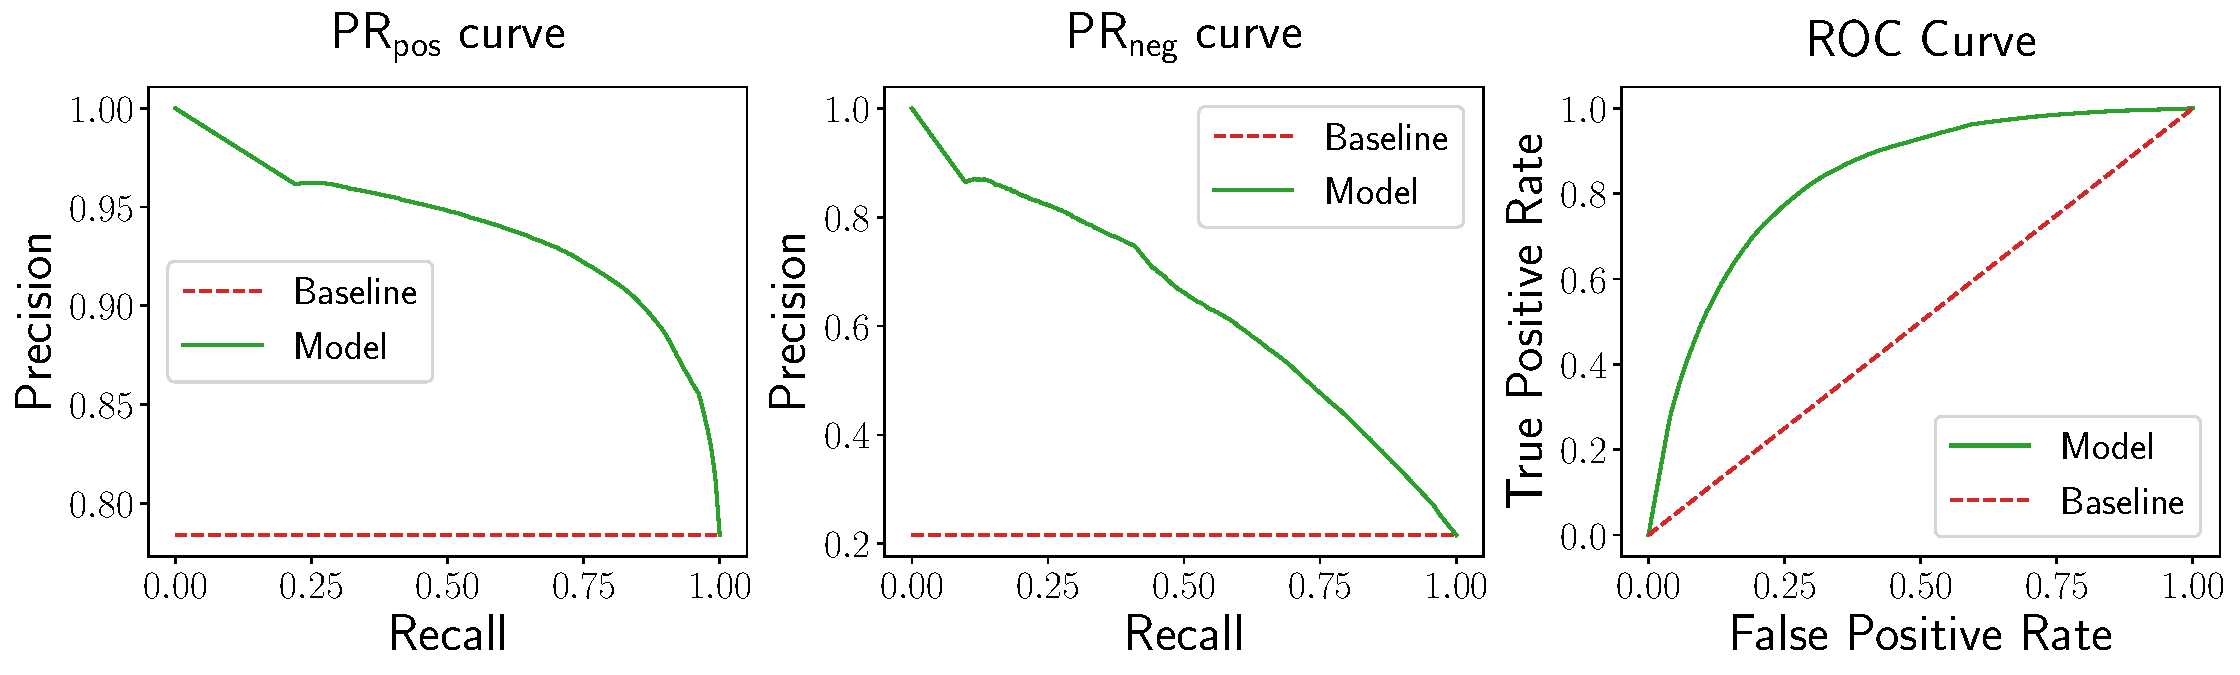
\includegraphics[width=0.7\textwidth]{../images/iterative_Balance.pdf}
        \caption{Plots for the Iterative Balance Model on the complete \wikirfa dataset}
        \label{fig:complete-iterative-balance}
    \end{figure}

    \begin{figure}[htp]
        \centering
        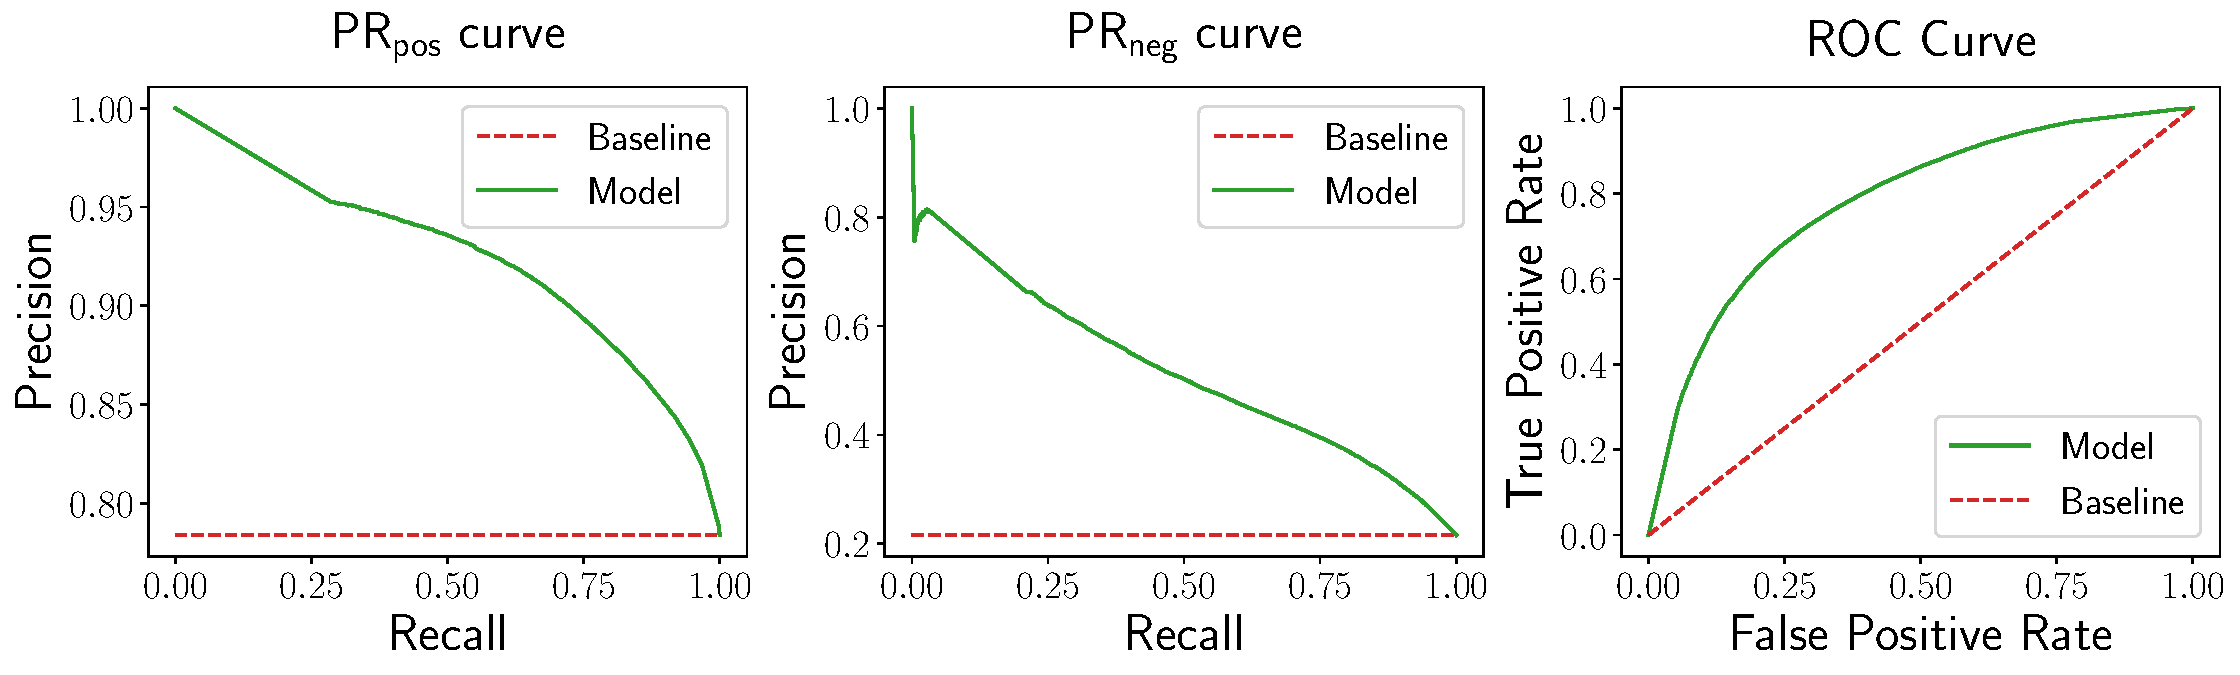
\includegraphics[width=0.7\textwidth]{../images/iterative_Status.pdf}
        \caption{Plots for the Iterative Status Model on the complete \wikirfa dataset}
        \label{fig:complete-iterative-status}
    \end{figure}   

\end{frame}

\begin{frame}
    \frametitle{}

    \centering \Large
    \emph{Questions or Comments}

\end{frame}

\bibliography{../sources}
\bibliographystyle{apalike}

\end{document}